%%=============================================================================
%% Opstelling en uitvoering van de testcases
%%=============================================================================

\chapter{Opstelling en uitvoering van de testcases}%
\label{ch:testcases}

Dit hoofdstuk beschrijft hoe de labo-omgevingen van de \emph{OLODs} \emph{Cybersecurity Advanced} en \emph{Infrastructure Automation} zijn herontworpen als \emph{PlantUML}-invoer (netwerk- en implementatiediagrammen) voor de \emph{converter}. Hierna wordt dan ook telkens beschreven welke \emph{Vagrant}- en \emph{Ansible}-uitvoer hier telkens uit ontstaat. De selectie van hosts en rollen is gebaseerd op de originele \emph{Vagrant}- en \emph{Ansible}-configuraties van de betrokken labo's, maar er zullen daarin beperkingen zijn wegens de scope van de \emph{Proof of Concept}.

\section{Werkwijze}%
\label{sec:werkwijze_testcases}

Voor elke testcase worden eerst de beheerde hosts uit de betrokken labo-omgevingen geïdentificeerd (op basis van de originele ``\texttt{vagrant-hosts.yml}'' en ``\texttt{inventory.yml}'') en vervolgens in het netwerkdiagram gedefinieerd.
Hosts die door de \emph{converter} niet ondersteund worden of niet tot de beheerde infrastructuur behoren zoals routers, workstations, de laptop van de gebruiker en VirtualBox-specifieke netwerkinfrastructuur (``\texttt{virtualbox\_nat\_gateway}'', ``\texttt{virtualbox\_nat\_dns}''), worden als niet-beheerd gemarkeerd (via ``\texttt{managed = false}'') in het netwerkdiagram.

Het implementatiediagram wordt daarna opgesteld via ``\texttt{node}''-definities voor elke beheerde host en ``\texttt{component}''-definities voor elke toegewezen rol.
De \emph{Ansible}-rollen worden gebaseerd op de originele hostvariabelen (``\texttt{host\_vars}'') en \emph{playbook} (``\texttt{site.yml}'') van de labo-omgeving en vervolgens gedefinieerd via de \emph{role identifiers} die opgelijst staan in het ``\texttt{role-config.yml}''-bestand van de \emph{converter} (zie \autoref{subsec:rolconfiguratie}).
Pijlverbindingen tussen rollen worden enkel opgenomen wanneer de \emph{converter} ze effectief herkent als mogelijke verbinding, namelijk \emph{DNS}-verbindingen (bijvoorbeeld ``\texttt{web.dns\_client --> dns.dns\_server\_primary}'') en \emph{Prometheus} scrape targets (bijvoorbeeld ``\texttt{mon.monitoring\_server --> web.node\_exporter}'').

Ten slotte wordt de \emph{converter} uitgevoerd op de opgestelde invoerbestanden en wordt de gegenereerde uitvoer beoordeeld aan de hand van de volgende criteria:
\begin{itemize}
    \item Zijn alle beheerde hosts aanwezig in de gegenereerde ``\texttt{vagrant-hosts.yml}''- en ``\texttt{inventory.yml}''-bestanden?
    \item Zijn de gegenereerde hostvariabelen correct en volledig ingevuld?
    \item Is de gegenereerde \emph{playbook} (``\texttt{site.yml}'') correct en sluit de uitvoervolgorde van de plays aan bij de verwachte afhankelijkheden?
    \item Kan de omgeving succesvol worden opgestart met het ``\texttt{vagrant up}''-commando zonder manuele aanpassingen achteraf?
\end{itemize}

\section{Testcase 1: \emph{Cybersecurity Advanced} (\emph{IaC-only mode})}%
\label{sec:testcase1}

Het \emph{OLOD} \emph{Cybersecurity Advanced} maakt gebruik van een labo-omgeving bestaande uit vier subnetten:

\begin{itemize}
    \item Een intern bedrijfsnetwerk (``\texttt{internal-company-lan}'', ``\texttt{172.30.0.0/16}'')
    \item Een gesimuleerd internetnetwerk (``\texttt{fake-internet}'', ``\texttt{192.168.62.0/24}'')
    \item Een thuisnetwerk van een medewerker (``\texttt{employee-home-lan}'', \\``\texttt{172.10.10.0/24}'')
    \item Een VirtualBox \emph{NAT}-netwerk die louter didactisch wordt voorgesteld (``\texttt{virtualbox\_nat}'', ``(\texttt{10.0.2.0/24})'')
\end{itemize}

De beheerde hosts omvatten:

\begin{itemize}
    \item De routers ``\texttt{companyrouter}'', ``\texttt{isprouter}'' (enkel voor het ``\texttt{fake-internet}''-netwerk) en ``\texttt{homerouter}''
    \item Een \emph{DNS}-server ``\texttt{dns}''
    \item Een webserver ``\texttt{web}''
    \item Een databank ``\texttt{database}''
    \item Twee werkstations ``\texttt{employee}'' en ``\texttt{remote-employee}''
\end{itemize}

Aangezien het \nameref{subsec:fullmode}-gebruiksscenario van de \emph{converter} slechts één beheerd subnet ondersteunt en de ``\texttt{role-config.yml}'' geen rollen voor routers of werkstations bevat, wordt deze testcase uitsluitend via de \nameref{subsec:iaconlymode} uitgevoerd. Deze modus produceert enkel een ``\texttt{vagrant-hosts.yml}''- en ``\texttt{Vagrantfile}''-bestand, zonder \emph{Ansible}-configuratie. Bijgevolg wordt er hier dus géén implementatiediagram opgesteld. De host ``\texttt{your-laptop}'' en de VirtualBox-specifieke netwerkinfrastructuur worden als niet-beheerd gemarkeerd.

\subsection{Invoer: netwerkdiagram}%
\label{subsec:testcase1_invoer}

Het opgestelde netwerkdiagram (``\texttt{nwdiag\_cybersec\_adv\_env.puml}'') bevat alle subnetten en (al dan niet beheerde) hosts uit de originele labo-omgeving.

\begin{codeblock}
    \lstinputlisting[language=plantuml]{../project_files/input/cybersec_adv_env/nwdiag_cybersec_adv_env.puml}
    \caption[Netwerkdiagram testcase 1 in tekstformaat (\emph{PlantUML})]{Tekstformaat (``\texttt{nwdiag\_cybersec\_adv\_env.puml}'') van het netwerkdiagram voor testcase 1 (\emph{Cybersecurity Advanced}).}
    \label{code:nwdiag_cybersec_adv}
\end{codeblock}

Dit bestand genereert via \emph{PlantUML} de volgende afbeelding.

\begin{figure}[H]
    \centering
    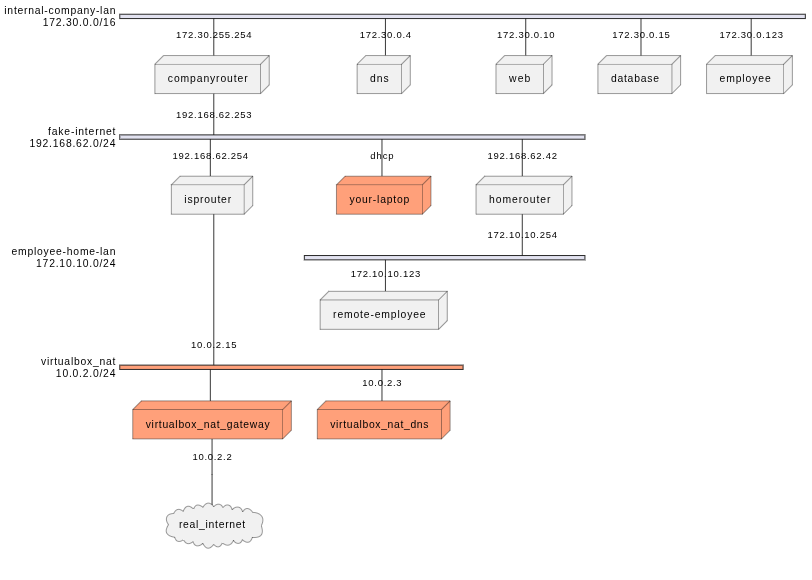
\includegraphics[width=\textwidth]{../graphics/nwdiag_cybersec_adv_env.png}
    \caption[Netwerkdiagram testcase 1 in afbeeldingsformaat (\emph{PlantUML})]{Afbeeldingsformaat van het netwerkdiagram voor testcase 1 (\emph{Cybersecurity Advanced}), gegenereerd door \emph{PlantUML}.}
    \label{fig:nwdiag_cybersec_adv}
\end{figure}

\subsection{Gegenereerde bestanden}%
\label{subsec:testcase1_gegenereerd}

De \emph{converter} genereert het ``\texttt{vagrant-hosts.yml}''-bestand in de uitvoermap. Dit bestand bevat voor elke beheerde host een entry met overeenkomend(e) IP-adres(sen) en werkgeheugen, afkomstig uit de ``\texttt{address}''- en ``\texttt{memory}''-attributen in het netwerkdiagram. De routers ``\texttt{companyrouter}'' en ``\texttt{homerouter}'' beschikken elk over meerdere netwerkinterfaces (één per verbonden subnet), wat resulteert in meerdere IP-adresregels per entry.

\begin{codeblock}
    \inputminted{yaml}{../project_files/output/cybersec_adv_env/vagrant-hosts.yml}
    \caption[Gegenereerde ``\texttt{vagrant-hosts.yml''} voor testcase 1]{De door de \emph{converter} gegenereerde \texttt{vagrant-hosts.yml} voor testcase 1 (\emph{Cybersecurity Advanced}).}
    \label{code:vagrant_hosts_cybersec}
\end{codeblock}

\subsection{Gekopieerde assets}%
\label{subsec:testcase1_assets}

Naast het gegenereerde ``\texttt{vagrant-hosts.yml}''-bestand kopieert de \emph{converter} ook een vooraf opgestelde ``\texttt{Vagrantfile}'' naar de uitvoermap. Deze leest de ``\texttt{vagrant-hosts.yml}'' in en voorziet voor elke entry de correcte \emph{Vagrant}-VM-configuratie, inclusief de VirtualBox-netwerkinstellingen.

\subsection{Beoordeling}%
\label{subsec:testcase1_beoordeling}

Alle beheerde hosts uit de originele labo-omgeving zijn aanwezig in de gegenereerde ``\texttt{\emph{Vagrant}-hosts.yml}''. De ``\texttt{address}''- en ``\texttt{memory}''-attributen uit het netwerkdiagram zijn correct overgenomen en omgezet tot de juiste waarden.
De Vagrant-omgeving kan worden opgestart met het ``\texttt{vagrant up}''-commando zonder verdere manuele aanpassingen.

Ter verduidelijking; de \emph{Vagrant}-VM's worden hier wel aangemaakt, maar zonder enige \emph{Ansible}-configuratie. De gegenereerde omgeving is bijgevolg niet functioneel equivalent aan de volledige originele labo-opzet: de subnetten zijn niet onderling verbonden via de routers (``\texttt{companyrouter}'', ``\texttt{isprouter}'', ``\texttt{homerouter}''), de \emph{firewall}- en \emph{NAT}-regels ontbreken, en er wordt geen software op onder andere de webserver en databank geïnstalleerd. Deze output kan wel als vertrekpunt gebruikt worden om manuele of aanvullende configuratie (al dan niet via \emph{Ansible}) nadien toe te passen.

\section{Testcase 2: \emph{Infrastructure Automation}, labo 2 (\emph{Full mode})}%
\label{sec:testcase2}

Het tweede labo van het \emph{OLOD} \emph{Infrastructure Automation} beschrijft het opzetten van een enkel lokaal netwerk (``\texttt{infra.lan}'', ``\texttt{172.16.0.0/16}'') met de volgende hosts:

\begin{itemize}
    \item een primaire \emph{DNS}-server (``\texttt{srv001}'')
    \item een secundaire \emph{DNS}-server (``\texttt{srv002}'')
    \item een \emph{DHCP}-server (``\texttt{srv003}'')
    \item een webserver (``\texttt{srv100}'')
\end{itemize}

De router ``\texttt{r001}'', gebruikerslaptop ``\texttt{your-laptop}'' en het werkstation ``\texttt{ws0001}'' worden niet door de \emph{converter} beheerd. Deze omgeving wordt opgezet via het \nameref{subsec:fullmode}-gebruiksscenario van de \emph{converter}.

\subsection{Invoer: netwerk- en implementatiediagram}%
\label{subsec:testcase2_invoer}

Het opgestelde netwerkdiagram (``\texttt{nwdiag\_infra\_auto\_lab\_2\_env.puml}'') bevat één beheerd subnet (``\texttt{infra.lan}''). De niet-beheerde hosts (``\texttt{r001}'', ``\texttt{your-laptop}'' en ``\texttt{ws0001}'') en het volledige ``\texttt{virtualbox\_nat}''-netwerk worden als niet-beheerd gemarkeerd.

\begin{codeblock}
    \lstinputlisting[language=plantuml]{../project_files/input/infra_auto_lab_2_env/nwdiag_infra_auto_lab_2_env.puml}
    \caption[Netwerkdiagram testcase 2 in tekstformaat (\emph{PlantUML})]{Tekstformaat (``\texttt{nwdiag\_infra\_auto\_lab\_2\_env.puml}'') van het netwerkdiagram voor testcase 2 (\emph{Infrastructure Automation}, labo 2).}
    \label{code:nwdiag_infra_auto_lab2}
\end{codeblock}

\begin{figure}[H]
    \centering
    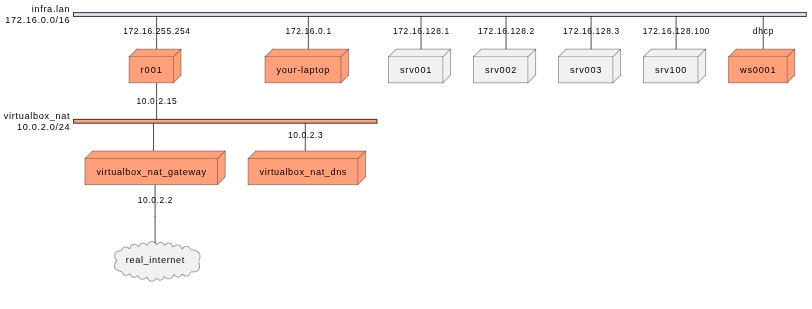
\includegraphics[width=\textwidth]{../graphics/nwdiag_infra_auto_lab_2_env.png}
    \caption[Netwerkdiagram testcase 2 in afbeeldingsformaat (\emph{PlantUML})]{Afbeeldingsformaat van het netwerkdiagram voor testcase 2 (\emph{Infrastructure Automation}, labo 2), gegenereerd door \emph{PlantUML}.}
    \label{fig:nwdiag_infra_auto_lab2}
\end{figure}

Het opgestelde implementatiediagram (``\texttt{uml\_infra\_auto\_lab\_2\_env.puml}'') stelt ``\texttt{node}''-definites op voor de vier beheerde hosts. De pijlverbindingen vanuit alle ``\texttt{dns\_client}''-componenten naar ``\texttt{srv001.dns\_server\_primary}'' en ``\texttt{srv002.dns\_server\_secondary}'' worden door de \emph{converter} gebruikt om de \emph{DNS}-serverconfiguratie en de \emph{DHCP}-subnettendefinitie correct in te vullen.

\begin{codeblockfixed}
    \begin{codeblock}
        \lstinputlisting[language=plantuml]{../project_files/input/infra_auto_lab_2_env/uml_infra_auto_lab_2_env.puml}
        \caption[Implementatiediagram testcase 2 in tekstformaat (\emph{PlantUML})]{Tekstformaat (``\texttt{uml\_infra\_auto\_lab\_2\_env.puml}'') van het implementatiediagram voor testcase 2 (\emph{Infrastructure Automation}, labo 2).}
        \label{code:uml_infra_auto_lab2}
    \end{codeblock}
\end{codeblockfixed}

\begin{figure}[H]
    \centering
    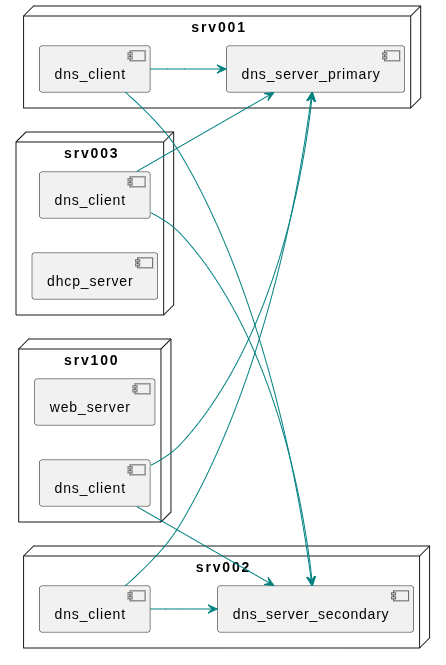
\includegraphics[width=.55\textwidth]{../graphics/uml_infra_auto_lab_2_env.png}
    \caption[Implementatiediagram testcase 2 in afbeeldingsformaat (\emph{PlantUML})]{Afbeeldingsformaat van het implementatiediagram voor testcase 2 (\emph{Infrastructure Automation}, labo 2), gegenereerd door \emph{PlantUML}.}
    \label{fig:uml_infra_auto_lab2}
\end{figure}

\subsection{Gegenereerde bestanden}%
\label{subsec:testcase2_gegenereerd}

De \emph{converter} genereert de volgende bestanden in de uitvoermap:

\begin{itemize}
    \item ``\texttt{vagrant-hosts.yml}'': de \emph{Vagrant}-VM-definities
    \item ``\texttt{ansible/inventory.yml}'': de \emph{Ansible}-\emph{inventory}
    \item ``\texttt{ansible/site.yml}'': de (hoofd-)\emph{playbook}
    \item ``\texttt{ansible/host\_vars/srv001.yml}'': de hostvariabelen voor ``\texttt{srv001}''
    \item ``\texttt{ansible/host\_vars/srv002.yml}'': de hostvariabelen voor ``\texttt{srv002}''
    \item ``\texttt{ansible/host\_vars/srv003.yml}'': de hostvariabelen voor ``\texttt{srv003}''
    \item ``\texttt{ansible/host\_vars/srv100.yml}'': de hostvariabelen voor ``\texttt{srv100}''
    \item ``\texttt{ansible/requirements.yml}'': de ``\emph{Ansible Galaxy}''-afhankelijkheden
\end{itemize}

De \emph{playbook} (``\texttt{site.yml}'') bevat plays in de volgorde bepaald door het topologisch sorteeralgoritme (zie \autoref{subsec:dynamische_bestanden}): hosts met ``\texttt{dns\_server\_primary}'' of ``\texttt{dns\_server\_secondary}'' worden vóór hosts met ``\texttt{dns\_client}'' geconfigureerd, overeenkomstig de ``\texttt{depends\_on}''-relaties in ``\texttt{role-config.yml}''.

\begin{codeblock}
    \inputminted{yaml}{../project_files/output/infra_auto_lab_2_env/ansible/site.yml}
    \caption[Gegenereerde ``\texttt{site.yml}'' voor testcase 2]{De door de \emph{converter} gegenereerde ``\texttt{site.yml}'' voor testcase 2 (\emph{Infrastructure Automation}, labo 2).}
    \label{code:site_infra_auto_lab2}
\end{codeblock}

\subsection{Gekopieerde assets}%
\label{subsec:testcase2_assets}

Naast de gegenereerde bestanden kopieert de \emph{converter} de volgende assets naar de uitvoermap:

\begin{itemize}
    \item ``\texttt{Vagrantfile}'': het standaard \emph{Vagrant}-sjabloon
    \item ``\texttt{scripts/}'': de \emph{Vagrant}-provisioneringsscripts
    \item ``\texttt{ansible/roles/web\_server}'': de voorgedefinieerde ``\texttt{web\_server}''-rol
    \item ``\texttt{ansible/roles/dns\_server}'': de voorgedefinieerde ``\texttt{dns\_server}''-rol (wordt voor zowel voor ``\texttt{dns\_server\_primary}'' als ``\texttt{dns\_server\_secondary}'' gebruikt)
    \item ``\texttt{ansible/roles/dns\_client}'': de voorgedefinieerde ``\texttt{dns\_client}''-rol
    \item ``\texttt{ansible/files/ca.crt}'', ``\texttt{ansible/files/ca.key}'', \\``\texttt{ansible/files/db.sql}'', ``\texttt{ansible/files/test.php}'': de statische bestanden benodigd voor de ``\texttt{web\_server}''-rol
\end{itemize}

\subsection{Beoordeling}%
\label{subsec:testcase2_beoordeling}

Alle vier beheerde hosts zijn aanwezig in de gegenereerde uitvoer. De \emph{DNS}-zone-informatie, de \emph{DHCP}-subnettendefinitie en de \emph{firewall}-poortenlijsten zijn correct afgeleid uit de diagraminformatie en het ``\texttt{role-config.yml}''-bestand.

De router ``\texttt{r001}'' is de voornaamste beperking van deze testcase: het doel van deze host wordt door de \emph{converter} niet ondersteund en is bijgevolg afwezig in de geproduceerde uitvoer. De beheerde hosts beschikken wel over internettoegang via hun eigen VirtualBox \emph{NAT}-interface, maar onderlinge routering is dus niet geconfigureerd. \emph{DNS}-queries tussen de hosts onderling blijven wel functioneel, aangezien deze via de gegenereerde \emph{DNS}-serverconfiguratie verlopen.

\section{Testcase 3: \emph{Infrastructure Automation}, labo 3 (\emph{Full mode})}%
\label{sec:testcase3}

Labo 3 van \emph{Infrastructure Automation} bouwt verder op de omgeving van labo 2 door een monitoring-server (``\texttt{srv004}'') toe te voegen. Op deze host wordt \emph{Prometheus} en \emph{Grafana} geïnstalleerd via de ``\texttt{monitoring\_server}''-rol. Op alle hosts worden daarnaast ook dienst-specifieke exporters voorzien.

\subsection{Invoer: netwerk- en implementatiediagram}%
\label{subsec:testcase3_invoer}

Het netwerkdiagram (``\texttt{nwdiag\_infra\_auto\_lab\_3\_env.puml}'') is een uitbreiding van het opgestelde netwerkdiagram uit testcase 2 met de toevoeging van de host ``\texttt{srv004}'' (met 2 \emph{CPU} cores en 2048 MB werkgeheugen).

\begin{codeblockfixed}
    \begin{codeblock}
        \lstinputlisting[language=plantuml]{../project_files/input/infra_auto_lab_3_env/nwdiag_infra_auto_lab_3_env.puml}
        \caption[Netwerkdiagram testcase 3 in tekstformaat (\emph{PlantUML})]{Tekstformaat (``\texttt{nwdiag\_infra\_auto\_lab\_3\_env.puml}'') van het netwerkdiagram voor testcase 3 (\emph{Infrastructure Automation}, labo 3).}
        \label{code:nwdiag_infra_auto_lab3}
    \end{codeblock}
\end{codeblockfixed}

\begin{figure}[H]
    \centering
    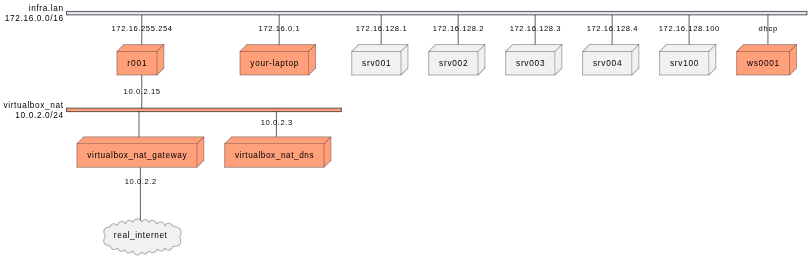
\includegraphics[width=\textwidth]{../graphics/nwdiag_infra_auto_lab_3_env.png}
    \caption[Netwerkdiagram testcase 3 in afbeeldingsformaat (\emph{PlantUML})]{Afbeeldingsformaat van het netwerkdiagram voor testcase 3 (\emph{Infrastructure Automation}, labo 3), gegenereerd door \emph{PlantUML}.}
    \label{fig:nwdiag_infra_auto_lab3}
\end{figure}

Het implementatiediagram (``\texttt{uml\_infra\_auto\_lab\_3\_env.puml}'') breidt het opgestelde implementatiediagram uit testcase 2 uit door de host/``\texttt{node}'' ``\texttt{srv004}'' toe te voegen, alsook dienst-specifieke exporterrollen voor elke ``\texttt{node}'':

\begin{itemize}
    \item ``\texttt{apache\_exporter}'' voor ``\texttt{srv100}''
    \item ``\texttt{bind\_exporter}'' voor ``\texttt{srv001}'' en ``\texttt{srv002}''
    \item ``\texttt{mysqld\_exporter}'' voor ``\texttt{srv100}''
    \item ``\texttt{node\_exporter}'' voor elke ``\texttt{node}'', inclusief ``\texttt{srv004}''
\end{itemize}

De pijlverbindingen vanuit ``\texttt{srv004.monitoring\_server}'' naar alle exporterrollen worden door de \emph{converter} gebruikt om de \emph{Prometheus} scrape targets automatisch op te bouwen (via de ``\texttt{prometheus\_scrape\_configs}''-variabele).

\begin{codeblock}
    \lstinputlisting[language=plantuml]{../project_files/input/infra_auto_lab_3_env/uml_infra_auto_lab_3_env.puml}
    \caption[Implementatiediagram testcase 3 in tekstformaat (\emph{PlantUML})]{Tekstformaat (``\texttt{uml\_infra\_auto\_lab\_3\_env.puml}'') van het implementatiediagram voor testcase 3 (\emph{Infrastructure Automation}, labo 3).}
    \label{code:uml_infra_auto_lab3}
\end{codeblock}

\begin{figure}[H]
    \centering
    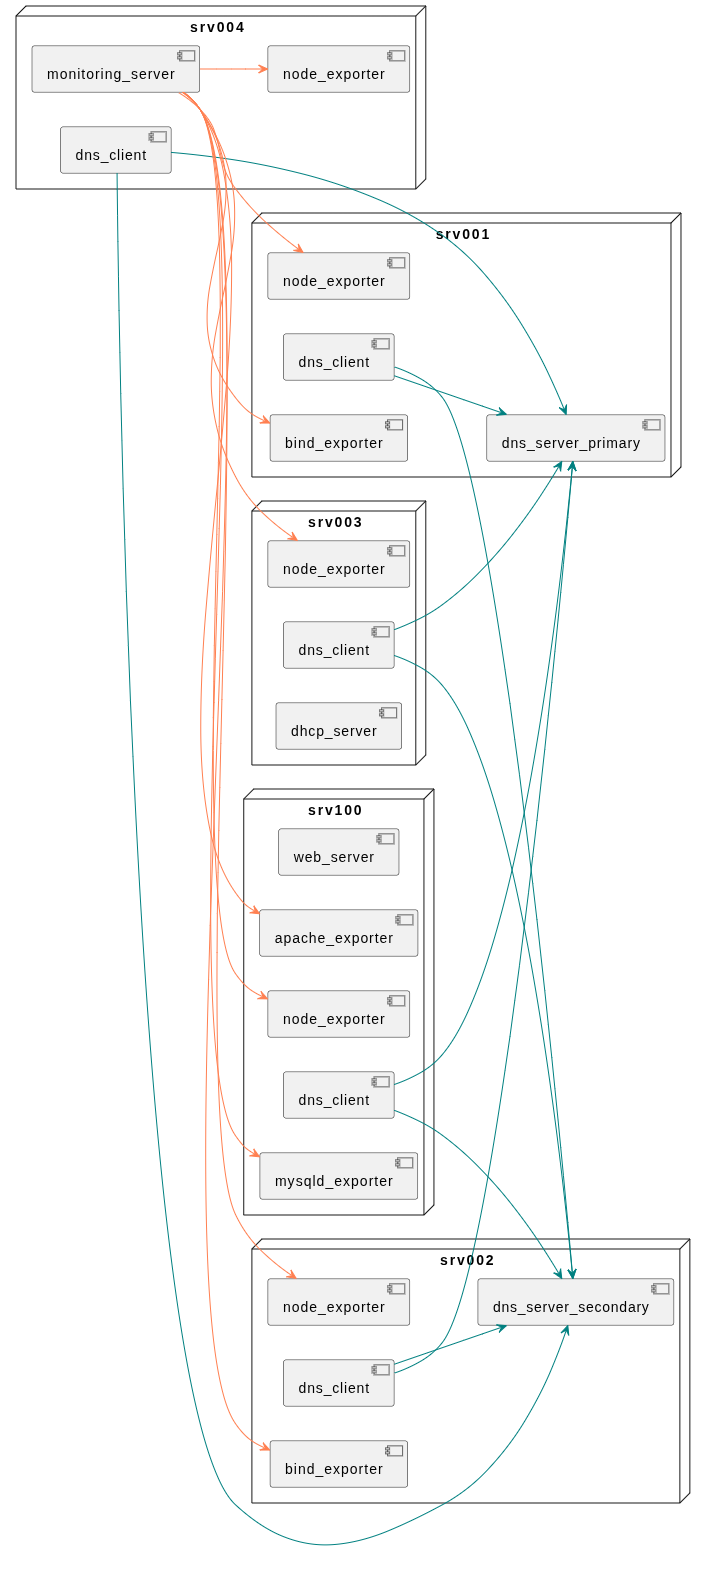
\includegraphics[width=.65\textwidth]{../graphics/uml_infra_auto_lab_3_env.png}
    \caption[Implementatiediagram testcase 3 in afbeeldingsformaat (\emph{PlantUML})]{Afbeeldingsformaat van het implementatiediagram voor testcase 3 (\emph{Infrastructure Automation}, labo 3), gegenereerd door \emph{PlantUML}.}
    \label{fig:uml_infra_auto_lab3}
\end{figure}

\subsection{Gegenereerde bestanden}%
\label{subsec:testcase3_gegenereerd}

Ten opzichte van testcase 2 zijn de volgende (extra) bestanden gegenereerd/uitgebreid:

\begin{itemize}
    \item ``\texttt{ansible/host\_vars/srv004.yml}'': de hostvariabelen voor ``\texttt{srv004}''
    \item Een uitgebreide ``\texttt{ansible/requirements.yml}'' met de \\``\texttt{prometheus.prometheus}''- en ``\texttt{grafana.grafana}''-``\emph{Ansible Galaxy}''-collecties
    \item De hostvariabelen van ``\texttt{srv001}'' en ``\texttt{srv002}'' zijn uitgebreid voor \\``\texttt{bind\_exporter}''
    \item De hostvariabelen van ``\texttt{srv100}'' zijn uitgebreid voor ``\texttt{apache\_exporter}'' en ``\texttt{mysqld\_exporter}''
\end{itemize}

De hostvariabelen van \texttt{srv004} bevatten de automatisch gegenereerde \\``\texttt{prometheus\_scrape\_configs}''-waarde, opgebouwd op basis van alle exporterverbindingen in het implementatiediagram.

\begin{codeblockfixed}
    \begin{codeblock}
        \inputminted{yaml}{../project_files/output/infra_auto_lab_3_env/ansible/host_vars/srv004.yml}
        \caption[Gegenereerde ``\texttt{host\_vars/srv004.yml''} voor testcase 3]{De door de \emph{converter} gegenereerde hostvariabelen voor \texttt{srv004}. De \texttt{prometheus\_scrape\_configs}-waarde is automatisch samengesteld op basis van de pijlverbindingen in het implementatiediagram.}
        \label{code:hostvars_srv004}
    \end{codeblock}
\end{codeblockfixed}

\subsection{Gekopieerde assets}%
\label{subsec:testcase3_assets}

Ten opzichte van testcase 2 worden de volgende extra assets gekopieerd:

\begin{itemize}
    \item ``\texttt{ansible/roles/monitoring\_server}'': \\de voorgedefinieerde ``\texttt{monitoring\_server}''-rol
    \item ``\texttt{ansible/files/grafana/default.yml}'': \\het configuratiebestand voor \emph{Grafana}
    \item ``\texttt{ansible/files/grafana/dashboards/apache\_exporter.json}'': \\het \emph{Grafana}-dashboard voor ``\texttt{apache\_exporter}''
    \item ``\texttt{ansible/files/grafana/dashboards/bind\_exporter.json}'': \\het \emph{Grafana}-dashboard voor ``\texttt{bind\_exporter}''
    \item ``\texttt{ansible/files/grafana/dashboards/mysqld\_exporter.json}'': \\het \emph{Grafana}-dashboard voor ``\texttt{mysqld\_exporter}''
    \item ``\texttt{ansible/files/grafana/dashboards/node\_exporter.json}'': \\het \emph{Grafana}-dashboard voor ``\texttt{node\_exporter}''
\end{itemize}

\subsection{Beoordeling}%
\label{subsec:testcase3_beoordeling}

De uitvoer voor labo 3 is functioneel equivalent aan de manueel opgestelde \emph{Ansible}-configuratie uit de originele labo-omgeving. Alle vijf beheerde hosts zijn aanwezig, de exporterconfiguraties zijn correct gegenereerd en de \emph{Prometheus} scrape-configuratie reflecteert nauwkeurig de verbindingen uit het implementatiediagram.

De beperking met betrekking tot ``\texttt{r001}'' geldt ook hier; zie \autoref{subsec:testcase2_beoordeling}. Daarnaast veronderstelt de gegenereerde ``\texttt{monitoring\_server}''-configuratie dat de \emph{DNS}-servers reeds operationeel zijn vóór de \emph{Prometheus}-installatie; dit is gegarandeerd door de ``\texttt{depends\_on}''-relaties in ``\texttt{role-config.yml}'' en straalt zich uit in de resulterende volgorde in ``\texttt{site.yml}''.